\documentclass[a4paper,11pt]{ctexart}
\usepackage{amsmath}
\usepackage{amssymb}
\usepackage{mathtools}
\usepackage[cdot,amssymb]{SIunits}
\usepackage{graphicx}
\usepackage{hyperref}
\usepackage{verbatim}
\usepackage{braket}

\allowdisplaybreaks

\author{Jiajun Ren \\
\href{mailto:jiajunren0522@gmail.com}{jiajunren0522@gmail.com}}
\title{aggregates Frenkel-Holstein model MPS solver}

\begin{document}
\maketitle
the object of each molecule (mol) has object phonon(ph), each mol has different
number of phonons, omegas, phonon levels, e-ph couplings, localexcitation
energies.

The structure of the MPS/MPO is 
\begin{figure}[htbp]
    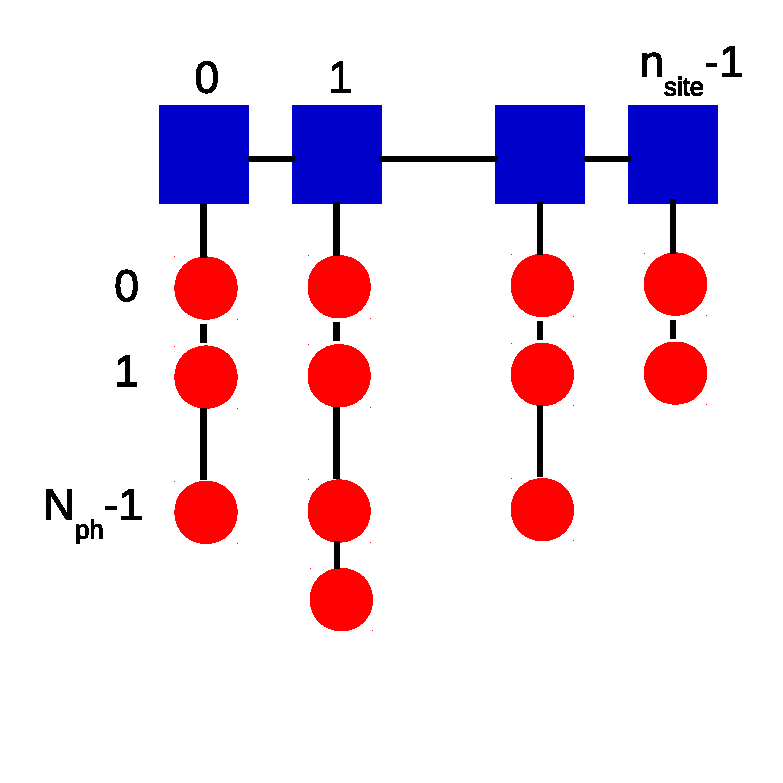
\includegraphics[width = \columnwidth]{structure.eps}  
    \caption{\label{fig:structure} tensor structure }
\end{figure}

\section{MPS structure}
\subsection{eMPS structure}
The eMPS structure is a list [] from mol 0 to mol nsites-1. \\
\# (e physical bond, left bond, right bond, e-ph bond) \\
eMPS(epb, eM, eM, ephM) \\

The eMPSdim is a list[] from 0 to nsites. \\
eMPSdim[0] = eMPSdim[nsites] = 1

\subsection{phMPS structure}
The phMPS structure is a nested list [[],[]] from mol 0 to mol nsites-1. each mol has a
sub list from phonon 0 to nphs-1.\\ (0 index is the left hand site) \\
\# (ph physical bond, left bond, right bond) \\
phMPS(ph.nlevels, phM, phM)
so the leftmost bond is linked to e site e-ph bond

The phMPSdim is a list [] from 0 to mol[imol].nphs
phMPSdim[mol[imol].nphs] = 1
    

\section{MPO structure}
We use the matrix representation to give the MPO
\subsection{eMPO structure}
eMPO is a list from mol 0 to mol nsites-1. \\
\# eMPO(bra, ket, l bond, r bond, e-pb bond)
eMPO(epb,epb,it denpends, it depends, 3)

eMPO structure (lbond, rbond, e-pb bond) is almost a matrix.
The third dimension only has one-line operator to connect phonon part operators.
\begin{gather}
MPO(k) = 
\begin{bmatrix}
    1 & 0 & 0  \\
    A_k & C_k & 0  \\
    B_k & D_k & 1  \\
\end{bmatrix}
\end{gather}

\begin{gather}
A(k) = 
\begin{bmatrix}
    J_{0k} a_k  \\
    J_{0k} a^\dagger_k \\
    ...  \\
    J_{k-1,k} a_k  \\
    J_{k-1,k} a^\dagger_k \\
\end{bmatrix}
\end{gather}

\begin{gather}
B(k) = 
\begin{bmatrix}
    e_k a^\dagger_k a_k \\
\end{bmatrix}
\end{gather}

\begin{gather}
C(k) = 
\begin{bmatrix}
    I  \\ 
\end{bmatrix}
\end{gather}

\begin{gather}
D(k) = 
\begin{bmatrix}
    0 & ... & 0 & a^\dagger_k & a_k  \\ 
\end{bmatrix}
\end{gather}

remember that the site 0 only has the last row operator,
the site nsites-1 only has the first columnn operator

The third dimenstion linked with phonon part is only attached to $B(k)$
It is 
\begin{gather}
\begin{bmatrix}
    B(k)  \\
    a^\dagger_k a_k \\
    1 \\
\end{bmatrix}
\end{gather}

The eMPOdim is a little bit complicated, because when we move to the right, we
add two operators $a^\dagger_k$ and $a_k$.
The eMPOdim is [1,4,6,8,...,2*nsites,1]
The third dimension is always 3.

\subsection{phMPO structure}
phMPO is a nested list [[]], from mol 0 to mol nsites-1. each mol has sub list
from phonon 0 to phonon nphs-1. 0 index is the left hand site. \\
\# (bra, ket, l bond, rbond)
phMPO(ph.nlevels, ph.nlevels, 3, 3).

The MPO in mol i and phonon n is that: \\
\begin{gather}
MPO(in) = 
\begin{bmatrix}
    1 & 0 & 0  \\
    g_{in} \omega_{in}(b^\dagger_{in}+b_{in}) & 1 & 0  \\
    \omega_{in} b^\dagger_{in}b_{in} & 0 & 1  \\
\end{bmatrix}
\end{gather}
The rightmost MPO has only the first column.
contract these MPOs we finally get
\begin{gather}
MPO(i) = 
\begin{bmatrix}
    1   \\
    \sum_n (g_{in} \omega_{in}(b^\dagger_{in}+b_{in}))   \\
    \sum_n (\omega_{in} b^\dagger_{in}b_{in})  \\
\end{bmatrix}
\end{gather}

The phMPOdim is a list [] from phonon 0 to nphs,
very simple: [3,3,3....,1]

When the temperature is high, then the phonon level should be increased, because
high level phonon excitation is probable. One the other hand, the emission
spectrum is not accurate, because without LF transformation, high level excited
state(high phonon level) is not discribed well, so when they are populated, the
result is probablly wrong. You can see in 1mol_1mode, the high level excited
states energy difference is wrong, not the phonon energy


for J aggregates, temperature effect is not so important. the effect temperature
is less than one single molecule.
far side band is not easy to occupied, because the close band density is large
if there is many molecules.

even in the zero temperature, J-aggregates 0-0 is much larger than the 0-1 peak.
Is it due to the addition of the dipole moment?

\end{document}
